\scanpage{10}
\mspage{2'}
Ces deux données pour le contour $C$ permettent de récupérer un graphe circularisé\unsure{s|,} $\Gamma$, ayant $\vec A$ comme ens des arêtes orientées, avec opérations $\sigma_A$, $\rho_S$ données ainsi :
\[
\left\{\begin{aligned}
\sigma_\Gamma&=\sigma_C\\
\rho_\Gamma&=\rho_C
\end{aligned}\right.
\]

\uline{En résumé} La catégorie des \inserted{$\underset{\cdot}{\unsure{c|C}}$}%
% Placement after des records horizontal position only; attachment remains unresolved.
 graphes combinatoires circularisés $\Gamma$ (sans sommet isolé) \inserted{$(\vec A\deleted{\unsure{_\Gamma}}(\Gamma),\rho_\Gamma,\sigma_\Gamma)$} est équivalente à celle des contours orientés, avec involution \inserted{\unsure{ss|s} pt fixe $\sigma_C$} sur l'ens des \uline{arêtes}, soit $C$ ($=A(C)$ ens des arêtes de $C$, $\rho_C$ rotation fondamentale de $C$, $\sigma_C$ involution sur $A(C)$). \deleted{\unsure{par} \inserted{\unsure{la|le|C}} \illegible{1}} \deleted{\unsure{p}} correspondance fondamentale \unsure{:|;}
\diagram{\begin{tikzcd}[row sep=large,column sep=large]
\vec A(\Gamma)&A(C)\arrow[l,"\sim"']\\
\sigma_\Gamma\arrow[r,leftrightarrow]&\unsure{\sigma_C|\rho_C}\\
\rho_{\unsure{\Gamma|\deleted{\Gamma}}}^{\unsure{r|\sigma|-1|\delta}}\sigma_\Gamma&\rho_C\arrow[l,*->]\\
\rho_\Gamma&\rho_C\sigma_C\arrow[l,*->]
\end{tikzcd}}
\margin{On appellera \unsure{cela|$C$ le} \uline{déploiement} du graphe plan donné}
\margin{$\rho_\Gamma^{\unsure{r|\sigma}}$ rotation-sommets pour la carte \unsure{actuel|actuelle} défini par $\Gamma$}

\figure{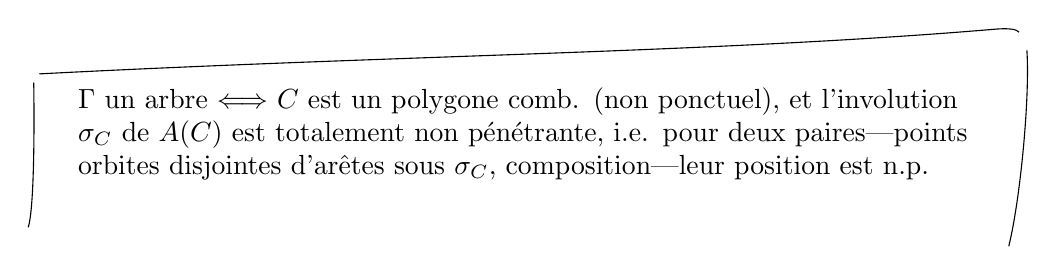
\begin{tikzpicture}[x=.01cm,y=-.01cm]\draw (238,1972) .. controls (700,1948) and (1100,1945) .. (1455,1915) .. controls (1470,1914) and (1480,1915) .. (1483,1919);\draw (231,1983) .. controls (232,2055) and (231,2145) .. (224,2167);\draw (1493,1942) .. controls (1497,2000) and (1485,2130) .. (1470,2191);\node[anchor=north west,align=left,text width=11.8cm] at (275,1977) {$\Gamma$ un arbre $\Longleftrightarrow$ $C$ est un polygone comb. (non ponctuel), et l'involution $\sigma_C$ de $A(C)$ est totalement non pénétrante, i.e. pour deux \deleted{\unsure{paires|points}} \inserted{orbites} disjointes d'arêtes sous $\sigma_C$, \unsure{composition|leur position} est n.p.};\end{tikzpicture}}
\margin{09}
